\ifdefined\isphone
  \documentclass[a6paper,11pt,oneside]{book}

\usepackage{algpseudocode}
\usepackage{algorithm}
\usepackage{amsfonts}
\usepackage{amsmath,amsthm,amssymb}
\usepackage{graphicx}
\usepackage{hyperref}
\usepackage{mathtools}
\usepackage{steinmetz}
\usepackage{fancyvrb}
\usepackage{textcomp}
\usepackage{gensymb}
\usepackage[normalem]{ulem}
\usepackage[T1]{fontenc}
\usepackage{cmap}
\usepackage{xspace}

\DeclareGraphicsExtensions{.pdf,.png,.jpg}

\newcommand{\mb}[1]{\ensuremath{\mathbb{{#1}}}}
\newcommand{\setof}[1]{\ensuremath{\left \{ #1 \right \}}}
\newcommand{\tuple}[1]{\ensuremath{\left \langle #1 \right \rangle }}

\DeclarePairedDelimiter{\ceil}{\lceil}{\rceil}
\DeclarePairedDelimiter{\floor}{\lfloor}{\rfloor}

\DeclareSymbolFont{bbold}{U}{bbold}{m}{n}
\DeclareSymbolFontAlphabet{\mathbbold}{bbold}

\newtheorem{statement}{Statement}
\newtheorem{rmk}{Remark}
\newtheorem{defi}{Definition}
\newtheorem{example}{Example}
\newtheorem{theorem}{Theorem}
\newtheorem{lemma}[theorem]{Lemma}
\newtheorem{proposition}[theorem]{Proposition}
\newtheorem{pf}[theorem]{Proof}
\newtheorem{corollary}[theorem]{Corollary}

% Differences
\usepackage[margin=5mm]{geometry}
\usepackage{tgheros}
\renewcommand*\familydefault{\sfdefault}

\else
  \documentclass[11pt,oneside]{book}

\usepackage{algpseudocode}
\usepackage{algorithm}
\usepackage{amsfonts}
\usepackage{amsmath,amsthm,amssymb}
\usepackage{graphicx}
\usepackage{hyperref}
\usepackage{mathtools}
\usepackage{steinmetz}
\usepackage{fancyvrb}
\usepackage{textcomp}
\usepackage{gensymb}
\usepackage[normalem]{ulem}
\usepackage[T1]{fontenc}
\usepackage{cmap}
\usepackage{xspace}

\DeclareGraphicsExtensions{.pdf,.png,.jpg}

\newcommand{\mb}[1]{\ensuremath{\mathbb{{#1}}}}
\newcommand{\setof}[1]{\ensuremath{\left \{ #1 \right \}}}
\newcommand{\tuple}[1]{\ensuremath{\left \langle #1 \right \rangle }}

\DeclarePairedDelimiter{\ceil}{\lceil}{\rceil}
\DeclarePairedDelimiter{\floor}{\lfloor}{\rfloor}

\DeclareSymbolFont{bbold}{U}{bbold}{m}{n}
\DeclareSymbolFontAlphabet{\mathbbold}{bbold}

\newtheorem{statement}{Statement}
\newtheorem{rmk}{Remark}
\newtheorem{defi}{Definition}
\newtheorem{example}{Example}
\newtheorem{theorem}{Theorem}
\newtheorem{lemma}[theorem]{Lemma}
\newtheorem{proposition}[theorem]{Proposition}
\newtheorem{pf}[theorem]{Proof}
\newtheorem{corollary}[theorem]{Corollary}

% Differences
\setlength{\textheight}{9.5in}
\setlength{\textwidth}{7.0in}
\setlength{\topmargin}{-0.75in}
\setlength{\oddsidemargin}{-0.25in}
\setlength{\evensidemargin}{0.75in}
\setlength{\parskip}{0.15in}
\setlength{\parindent}{0in}

\fi

\begin{document}

% Info section

\title{SE 350 End of Term Notes}

\author{
    Craig, Shale\\
    \texttt{sakcraig@uwaterloo.ca}
}
\maketitle

% Note: uncomment these if I add them
\tableofcontents
% \listofAlgorithms
% \listoffigures

\chapter{Memory}
\label{cha:memory}

    \section{Paging/Segmentation} % (fold)
    \label{sec:paging_segmentation}
        \subsection{Paging} % (fold)
        \label{subsec:paging}
            Paging allows memory to be comprised of fixed-size blocks that are
            addressed by virtual addresses that are page numbers and an offset. Each
            page can be anywhere in main memory.

            \subsection{Address Translation} % (fold)
            \label{subsec:address_translation}
            Address translation (logical, not physical addresses) allow us to use
            non-contiguous memory layouts, which allows processes to run without
            being fully resident in memory.

            Execute code. Once program tries to read/exec instructions not in RAM,
            we page fault, block, read data, then resume.

            Virtual Addresses are tuples of $\tuple{\text{Page \#}, \text{Offset}}$.
            We look up the Page Number + Page Table Pointer in the Page Table, which
            gives us the Frame \#. Combine (by a bitmask) the two points, and
            you get the physical address of the memory in main memory.

            Address Translation (i.e. a root page table) allows us to have large
            page tables, and keep some of the page tables in main memory while they
            are not being accessed.

            The downside of Page Tables is that Page Table size is proportional to
            the virtual address space.
            % subsection address_translation (end)

            \subsection{Segmentation} % (fold)
            \label{subsec:segmentation}
            Allows the programmer to view memory as multiple address spaces or
            segments. We can now share data among processes, and protect segments
            from data modification.

            Segmentation is pretty much the same as virtual addressing, except the
            segment table contains the base address and is added to the offset.

            % subsection segmentation (end)
            \subsection{Combined Paging and Segmentation} % (fold)
            \label{subsec:combined_paging_and_segmentation}
            Paging is transparent to the programmer while Segmentation is
            visible to the programmer.

            See figure \ref{fig:address_translation_and_segmentation} for more
            information.
            \begin{figure}[h]
                \label{fig:address_translation_and_segmentation}
                \centering
                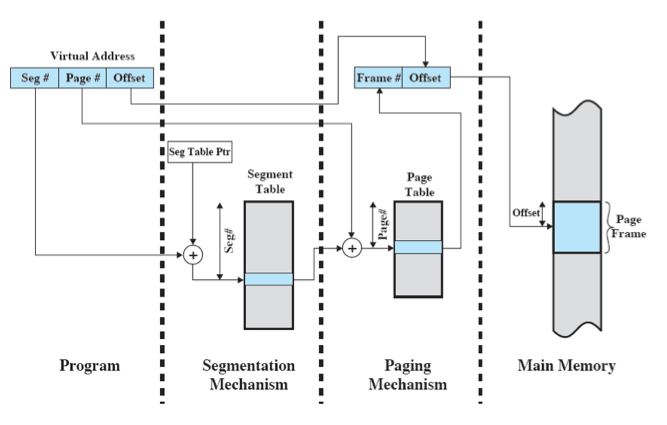
\includegraphics[scale=0.5,keepaspectratio]{images/address-translation-and-segmentation.png}
            \end{figure}

            % subsection combined_paging_and_segmentation (end)
    % section paging_segmentation (end)
    \section{Replacement Strategies} % (fold)
    \label{sec:replacement_allocation_strategies}
        \begin{itemize}
            \item Least Recently Used
            \item First-in, First-Out
            \item Clock Policy
            \item Page Buffering
        \end{itemize}
    \subsection{Page Buffering} % (fold)
    \label{subsec:page_buffering}
        Memory pages are cached and are placed into a ``free page'' or
        ``modified'' page list if they have or haven't been modified
        respectively. This is done so the OS can revive these pages from the
        list if space becomes available.
    % subsection page_buffering (end)
    % section replacement_allocation_strategies (end)

    \section{Page Size v.s. Page Faults} % (fold)
    \label{sec:page_size_v_s_page_faults}
    By having an smaller page size, all parts of the pages in memory will
    be relevant to the process in recent references. If they are bigger, there
    will be ``useless'' portions that aren't used
    % section page_size_v_s_page_faults (end)

    \section{Working Set v.s. Resident Set} % (fold)
    \label{sec:working_set_v_s_resident_set}
    Resident set is the portion of a process that is in main memory.
    The smaller the resident set size, the higher number of processes that can
    be in memory.
    Once it is past a certain size, there is no real gain from a large resident
    set.

    The working set is the set of pages of the process that have been referenced
    in the last $t$ time.

    % section working_set_v_s_resident_set (end)
    \section{Calculating the Resident Set Size} % (fold)
    \label{sec:calculating_the_resident_set_size}
    Variable allocation means the size of the working set for one process is
    fixed with respect to time.
    Variable allocation means the size of the working set for one process varies
    with respect to time.

    There are three main types of allocation strategies:
    \begin{itemize}
        \item Fixed Allocation, Local Scope:

            Decide before how big the working set should be, then execute under
            that decision.

        \item Variable Allocation, Local Scope:

            New processes get a working set size based on a heuristic.
            Page faults result in pages from the current (local) process's
            working set being kicked out.

        \item Variable Allocation, Global Scope:

            New processes get a working set size based on a heuristic.
            Page faults result in pages from any (i.e. global) process's working
            set being kicked out.
    \end{itemize}
    % section calculating_the_resident_set_size (end)
    \section{Principle of Locality} % (fold)
    \label{sec:principle_of_locality}
    Stuff you need in the future is close to stuff you needed in the past.

    % section principle_of_locality (end)
\chapter{Simultaneous Execution} % (fold)
\label{cha:simultaneous_execution}

    \section{Preconditions for Deadlock} % (fold)
    \label{sec:preconditions_for_deadlock}
    Preconditions for deadlock are as follows:
    \begin{itemize}
        \item Mutual Exclusion (i.e. no way to ensure processes use resources
        one at a time)
        \item Hold-And-Wait
        \item No preemption (with respect to resources)
        \item Circular wait
    \end{itemize}
    % section preconditions_for_deadlock (end)

    \section{Semaphores, Monitors, etc} % (fold)
    \label{sec:semaphores_monitors_etc}
        \subsection{Mutexes} % (fold)
        \label{subsec:mutexes}
            Special machine instructions allow us to test and set a variable in
            a single machine instruction (atomically).

            \begin{verbatim}
                boolean testSet(int i):
                    if (i == 0):
                        i = 1
                        return true
                    else:
                        return false

                void exchange(int register, int memory):
                    temp = memory
                    memory = register
                    register = temp
            \end{verbatim}

            This is simple and applicable to any number of processes on single
            or multiple processors, but it does busy-waiting and can allow
            starvation if there are multiple waiting processes.
        % subsection mutexes (end)
        \subsection{Semaphores} % (fold)
        \label{subsec:semaphores}
            Semaphores are special variables that are used for signaling.
            Semaphores are initialized to a nonnegative number, generally the
            maximum number of concurrent accesses.
            ``semWait'' decrements the value, ``semSignal'' increments the
            semaphore value.
            \begin{verbatim}
                void semWait(semaphore s):
                    s.count--
                    if (s.count < 0):
                        s.queue.push(getCurrentProcess())

                void semSignal(semaphore s):
                    s.count++
                    if (s.count <= 0):
                        p = s.queue.pop()
                        p.makeReady()
            \end{verbatim}
            Binary semaphores are the same, but they only take on binary values.
            \begin{verbatim}
                void semWaitB(binary_semaphore s):
                    if (s.value == 1):
                        s.value = 0
                    else:
                        s.queue.push(getCurrentProcess())

                void semSignalB(binary_semaphore s):
                    if (s.queue.isEmpty()):
                        s.value = 1
                    else:
                        p = s.queue.pop()
                        p.makeReady()
            \end{verbatim}
        % subsection semaphores (end)
    % section semaphores_monitors_etc (end)

    \section{Amdhal's Law} % (fold)
    \label{sec:amdhal_s_law}
    As the level of Multiprogramming increases, the returns will become
    asymptotically faster, but the limit will be constant. This is because there
    is a limited set of instructions that can be run at the same time.
    % section amdhal_s_law (end)

    \section{Scheduling Algorithms} % (fold)
    \label{sec:scheduling_algorithms}
    \begin{itemize}
        \item Rate Monotonic

            Lower bound on schedulable utilization = 0.693.
            Highest-priority task is the one with the shortest period.

        \item Earliest Deadline First:

            Can schedule a CPU utilization of 1.
            Highest-priority task is the one with the next deadline.
    \end{itemize}
    % section scheduling_algorithms (end)

% chapter simultaneous_execution (end)
\chapter{Other} % (fold)
\label{cha:other}
    \section{States for Processes} % (fold)
    \label{sec:states_for_processes}
    \begin{itemize}
        \item New
        \item Running
        \item Ready
        \item Blocked
        \item Ready-suspend
        \item Blocked-suspend
        \item Exit
    \end{itemize}
    % section states_for_processes (end)

% chapter other (end)

\end{document}